% !TEX encoding = UTF-8
% !TEX TS-program = pdflatex
% !TEX root = rel_datamining.tex
% !TEX spellcheck = it-IT

\section{Introduzione}

\subsection{Descrizione del dataset}

Il dataset contiene 26729 osservazioni relative agli animali che hanno lasciato il rifugio per animali della città di Austin nel periodo che va dall'Ottobre 2013 a Marzo 2016.
L'obiettivo è quello di utilizzare i dati del dataset per prevedere quale sarà il destino dei nuovi animali che verranno accolti nel centro.

I dati sono forniti da Kaggle per la competizione ``\textit{Shelter Animal Outcomes}''\footnote{\url{https://www.kaggle.com/c/shelter-animal-outcomes}} e, trattandosi di una sfida, viene fornito anche un secondo dataset di 11456 osservazioni, per le quali non è nota la variabile risposta, che deve essere utilizzato per fornire al sito le proprie previsioni, al fine di stilare una classifica.

\subsection{Descrizione delle variabili}

Il dataset è composto da 10 variabili che descrivono lo stato dell'animale quando ha lasciato il rifugio.
Più nel dettaglio:

\begin{itemize}
	\item \texttt{AnimalID}: codice univoco che viene affidato all'animale quando è entrato nel rifugio. Nel dataset principale viene fornito sotto forma di stringa, mentre nel dataset secondario viene fornito come numero intero.
	\item \texttt{Name}: nome dell'animale. Nel dataset principale ci sono 7691 animali senza un nome.
	\item \texttt{DateTIme}: data e ora in cui l'animale ha lasciato il rifugio. \`{E} espressa nel formato \texttt{aaaa-mm-gg hh:mm:ss}.
	\item \texttt{Outcome}: variabile risposta, ha 5 possibili valori:
		\begin{itemize}
			\item \textit{Adoption}: 10769 osservazioni.
			\item \textit{Died}: 197 osservazioni.
			\item \textit{Euthanasia}: 1555 osservazioni.
			\item \textit{Return to owner}: 4786 osservazioni.
			\item \textit{Transfer}: 9422 osservazioni.
		\end{itemize}
	\item \texttt{OutcomeSubtype}: variabile che descrive perché l'animale ha fatto quella particolare fine. Ci sono 17 possibili valori per questa variabile e per 13612 non è disponibile. Questa variabile non è presente sul dataset secondario.
	\item \texttt{AnimalType}: tipo dell'animale, può essere un cane o un gatto.
	\item \texttt{SexuponOutcome}: sesso dell'animale, comprende anche l'informazione se l'animale è stato castrato o meno. In tutto ci sono 6 possibili valori per questa variabile.
	\item \texttt{AgeuponOutcome}: età dell'animale quando ha lasciato il rifugio, viene espressa utilizzando una stringa che descrive l'età, ad esempio: \textit{2 years, 1 week, ecc.}
	\item \texttt{Breed}: razza dell'animale. Comprende anche l'informazione se l'animale è un incrocio di più razze e in qualche caso specifica anche la seconda razza. In tutto ci sono 1380 possibili valori.
	\item \texttt{Color}: colore del pelo dell'animale. Comprende anche le informazioni relative al pelo e ad un eventuale colore secondario. In tutto ci sono 336 possibili valori.
\end{itemize}

La struttura del dataset una volta caricato in R è la seguente:

\begin{verbatim}
'data.frame':	26729 obs. of  10 variables:
$ AnimalID      : Factor w/ 26729 levels "A006100","A047759",..
$ Name          : Factor w/ 6375 levels ""," Joanie"," Mario",..
$ DateTime      : Factor w/ 22918 levels "2013-10-01 09:31:00",..
$ OutcomeType   : Factor w/ 5 levels "Adoption","Died",..
$ OutcomeSubtype: Factor w/ 17 levels "","Aggressive",..
$ AnimalType    : Factor w/ 2 levels "Cat","Dog"
$ SexuponOutcome: Factor w/ 6 levels "","Intact Female",..
$ AgeuponOutcome: Factor w/ 45 levels "","0 years","1 day",..
$ Breed         : Factor w/ 1380 levels "Abyssinian Mix",..
$ Color         : Factor w/ 366 levels "Agouti","Agouti/Brown Tabby",..
\end{verbatim}

Inoltre, andando a tracciare il grafico con le proporzioni delle varie classi in base al tipo di animale (Figura \ref{fig-animals}) è possibile osservare che per i cani è più probabile che siano recuperati dai propri padroni rispetto ai gatti, mentre per i gatti è più probabile che vengano trasferiti.

\begin{figure}[htbp]
	\centering
	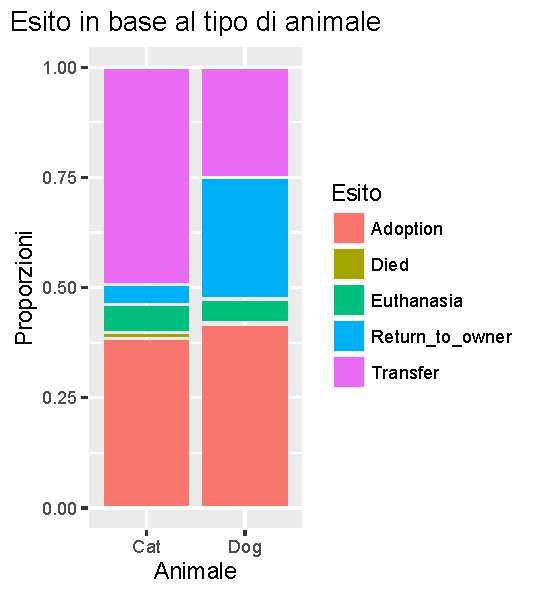
\includegraphics[width=0.4\textwidth]{./grafici/esito_animal.pdf}
	\caption{Esito in base al tipo di animale}\label{fig-animals}
\end{figure}

\subsection{Software utilizzato}

Nella realizzazione del progetto è stato utilizzato l'ambiente R in versione 3.2.4, esteso con alcune librerie:

\begin{itemize}
	\item \texttt{ggplot2}: per la rappresentazione dei grafici.
	\item \texttt{dplyr}: per la manipolazione dei dati.
	\item \texttt{nnet}: reti neurali e regressione logistica.
	\item \texttt{GAM}: GAM.
	\item \texttt{earth}: MARS.
	\item \texttt{randomForest}: random forest.
	\item \texttt{tree}: alberi di classificazione.
	\item \texttt{ada}: Boosting.
\end{itemize}

Tutte le librerie sono disponibili su CRAN mentre il codice del progetto è disponibile su GitHub all'indirizzo \url{https://github.com/GiacomoManzoli/AnimalShelter}.

\todo{aggiornare le librerie, manca quella del Bagging}